%%%%%%%%%%%%%%%%%%%%%%%%%%%%%%%%%%%%%%%%%%%%%%%%%%%%%%%%%%%%%%%%%%%%%%%%%%%%%%%%%%%%%%%%%%%%%%%%%%%%%
%
%   Version     : 2.0
%
%   Filename    : main.tex
%
%   Description : This is the main file for the LaTeX thesis proposal document template.
%                 The template is intended for use by BSCS students. 
%
%                It is assumed that you can learn how to use LaTeX on your own.
%                Please check/read the following online LaTeX book:
%
%                                 http://en.wikibooks.org/wiki/LaTeX
%     
%   Author      : Florante R. Salvador
%
%   Contributors: 1.  Karlo Campos 
%                     a. margin settings for DLSU thesis paper 
%   
%   Notes       : Please email florante.salvador@dlsu.edu.ph for comments, suggestions, ideas etc.
%
%   Reference:
%
%
%   History/Updates:
%      March 12, 2009 -- created version 1.0 for release to CSC701M (Methods of Research) students
%      May 30, 2009   -- updated Title page and Abstract for undergrad ST students
%
%      Feb 27, 2015 -- Created Version 2 (major overhaul): changed class to report, created a figures folder, 
%                               removed unnecessary packages, added new comments  based on Ethel Ong's slides
%
%%%%%%%%%%%%%%%%%%%%%%%%%%%%%%%%%%%%%%%%%%%%%%%%%%%%%%%%%%%%%%%%%%%%%%%%%%%%%%%%%%%%%%%%%%%%%%%%%%%%%%

%%%%%%%%%%%%%%%%%%%%%%%%%%%%%%%%%%%%%%%%%%%%%%%%%%%%%%%%%%%%%%%%%%%%%%%%%%%%%%%%%%%%%%%%%%%%%%%%%%%%%%%%%%%%%%%%%%%%%%%
%
%  Filename   : preamble.tex
%
%  Description: Preamble file to :
%               a. specify related packages
%               b. set margins, commands, etc.
%
%  Note       : Edit the margin settings for your own printer
%                  You may add your own commands, environments (it is assumed that you know what you're doing.)
%
%%%%%%%%%%%%%%%%%%%%%%%%%%%%%%%%%%%%%%%%%%%%%%%%%%%%%%%%%%%%%%%%%%%%%%%%%%%%%%%%%%%%%%%%%%%%%%%%%%%%%%%%%%%%%%%%%%%%%%%

%\documentclass[12pt,titlepage,onepage, letterpaper]{article}

\documentclass[12pt,titlepage,onepage, letterpaper]{report}


%
%-- specify related packages
%

%
% \usepackage[utf8x]{inputenc}
%

\usepackage{apacite}           %-- APA style citation 
                               %-- refer to http://www.ctan.org/tex-archive/biblio/bibtex/contrib/apacite/

%
%  \usepackage{ucs}
%


\usepackage{amsmath}           %-- American Math Society packages
\usepackage{amsfonts}
\usepackage{amssymb}


\usepackage{graphicx}          %-- graphicx package needed for including figures in JPG or PNG format
 
%
%\usepackage{graphics}          %-- graphics related package (this was commented out) use when image is in EPS format
%
\usepackage{longtable}
\usepackage{lscape}
\usepackage{tabu}
\usepackage{verbatim}          %-- this package allows you to have multiple lines of comments by
                               %-- example:
                               %   \begin{comment}
                               %        ...your text here...
                               %   \end{comment}  

\usepackage{color}             %-- allows use of color with text
                               %-- example:  \textcolor{red}{This is the colored text in red.}
\usepackage{graphicx}
\usepackage{url}  %-- allows use of URLs example: \url{https:\ccs1.dlsu.edu.ph}


%
%-- set margins,  you may need to edit this for your own printer
%
\topmargin 0.0in
\oddsidemargin 0.0in
\evensidemargin 0.0in

\voffset 0.0in
\hoffset 0.5625in

\textwidth 5.75in
\textheight 8.5in


\parskip 1em
\parindent 0.25in

\bibliographystyle{apacite}            %-- use APA citation scheme

\hyphenation{ana-lysis know-ledge}     %-- LaTeX may not hyphenate correctly some words you use in your document
                                       %-- use \hyphenation to instruct LaTeX how to do it correctly, example above

\newcommand{\degree}{^{\circ}}         %-- use \newcommand to create your own "commands"
                                       %-- \newcommand works like the #define you learned in your COMPRO1 class
\usepackage{textcomp}
\newcommand*\vtick{\textquotesingle}
\newcommand{\etal}{et al.}


%\newcommand{\sinag}{\emph{Sinag}}
%\newcommand{\sinagtwo}{\emph{Sinag2}}

\newcommand{\figref}[1]{Figure \ref{#1}}
\newcommand{\appref}[1]{Appendix \ref{#1}}

%-- \newcommand{\Section}[1]{\section{#1}\setcounter{figure}{0}\setcounter{table}{0}}

%\newcommand{\shade}{\multicolumn{1}{|>{\columncolor[gray]{0.25}}c|}{}}
%\newcommand{\tableheader}[1]{\rowcolor{black}\color{white}{#1}}
%\newcommand{\cell}[2]{\multicolumn{1}{#1}{#2}}
%\newcommand{\definition}[2]{\textbf{\textit{#1}} --- #2}
%\newcommand{\itembit}[1]{\item \textbf{\textit{#1}}}
%\newcommand{\sgdef}[2]{\parbox[t][][t]{1.75in}{\textbf{#1}} \> \parbox[t][][t]{4.0in}{#2}\\\\}

%\newenvironment{sinagglossary}{\begin{flushleft}
%\begin{tabbing}
%\hspace{1.75in}\=\\}{\end{tabbing}\end{flushleft}}

\newcommand{\thestitle}[1]{{\Large \textsc{#1}}}


%---
%  \renewcommand{\thefigure}{\thesection.\arabic{figure}}
%  \renewcommand{\thetable}{\thesection.\arabic{table}}
%  \renewcommand{\contentsname}{Table of Contents}




                %-- includes LaTeX source file for the preamble 
                                  %-- include packages, sets the margin sequence, and many more... 
                                  %-- your job: check if the settings are suitable for your own printer

\graphicspath{{figures/}}  %-- figures is the name of the folder containing images JPG or PN

\begin{document}

%%%%%%%%%%%%%%%%%%%%%%%%%%%%%%%%%%%%%%%%%%%%%%%%%%%%%%%%%%%%%%%%%%%%%%%%%%%%%%%%%%%%%%%%%%%%%%%%%%%%%%
%
%   Filename    : title_page.tex 
%
%   Description : This file will contain your Title Page.
%                 
%%%%%%%%%%%%%%%%%%%%%%%%%%%%%%%%%%%%%%%%%%%%%%%%%%%%%%%%%%%%%%%%%%%%%%%%%%%%%%%%%%%%%%%%%%%%%%%%%%%%%%

\begin{titlepage}
\centering


%-- **EDIT** the following line to indicate your thesis title
\thestitle{Effects of Different Parameters on the Results of Community Detection Algorithms}

\vspace{1.75cm}
A Partial Thesis Document\\
Presented to\\
the Faculty of the College of Computer Studies\\
De La Salle University Manila

\vspace{1.75cm}
In Partial Fulfillment\\
of the Requirements for the Degree of\\
Bachelor of  Science in Computer Science

\vspace{1.75cm}
by\\
%-- **EDIT** the following line to indicate your name 
\vspace{1cm}

FERNANDEZ, Ryan Austin \\
POBLETE, Clarisse Felicia M.  \\
SAN PEDRO, Marc Dominic  \\
TAN, Johansson E.  \\

\vspace{1.75cm}
%-- **EDIT** the following line to indicate your adviser's name 
Charibeth K. CHENG \\
Adviser

\vspace{1.75cm}
\today
\end{titlepage}
              %-- includes LaTeX source file for the Title Page 
                                  %-- your job: **EDIT THIS FILE ** to indicate your own title, name, and thesis adviser's name

%%%%%%%%%%%%%%%%%%%%%%%%%%%%%%%%%%%%%%%%%%%%%%%%%%%%%%%%%%%%%%%%%%%%%%%%%%%%%%%%%%%%%%%%%%%%%%%%%%%%%%
%
%   Filename    : abstract.tex 
%
%   Description : This file will contain your abstract.
%                 
%%%%%%%%%%%%%%%%%%%%%%%%%%%%%%%%%%%%%%%%%%%%%%%%%%%%%%%%%%%%%%%%%%%%%%%%%%%%%%%%%%%%%%%%%%%%%%%%%%%%%%

\begin{abstract}
Social media has become a resource for data in the past years. Community detection in social media has become 
a popular field of study because of the large volume of data that could be extracted. This study aims to 
determine which combination of community detection algorithms and similarity parameters can produce the best
communities in Facebook and Twitter and to produce a visualization of the communities. Multiple iterations 
of community detection will be performed for each selected combination of algorithm and parameter. This study 
will also attempt to delve into the domain of Facebook community detection, a domain which has not been 
adequately explored. The results of this study can improve community detection in the future by determining 
the algorithm and parameter that would produce the best communities. This also means that, using the generated
visualization, meaningful data can already be extracted, which can be used by businesses or politicians to
determine patterns in their target audience.

\begin{flushleft}
\begin{tabular}{lp{4.25in}}
\hspace{-0.5em}\textbf{Keywords:}\hspace{0.25em} & Social networks, community detection, sentiment analysis\\
\end{tabular}
\end{flushleft}
\end{abstract}
                %-- this is the Abstract page
                                  %-- your job: **EDIT THIS FILE** to indicate your own abstract
\pagenumbering{roman}             %-- this will number pages as i, ii, iii, etc...
\setcounter{page}{2}

\tableofcontents                  %-- this command is used to generate the Table of Contents
\newpage
\listoffigures                    %-- this command is used to generate List of Figures

\newpage                       
\listoftables                     %-- this command is used to generate List of Tables

\newpage

\pagenumbering{arabic}            %-- this will number pages as 1, 2, 3, etc...
\setcounter{page}{1}              


%%%%%%%%%%%%%%%%%%%%%%%%%%%%%%%%%%%%%%%%%%%%%%%%%%%%%%%%%%%%%%%%%%%%%%%%%%%%%%%%%%%%%%%%%%%%%%%%%%%%%%
%
%   Filename    : chapter_1.tex 
%
%   Description : This file will contain your Research Description.
%                 
%%%%%%%%%%%%%%%%%%%%%%%%%%%%%%%%%%%%%%%%%%%%%%%%%%%%%%%%%%%%%%%%%%%%%%%%%%%%%%%%%%%%%%%%%%%%%%%%%%%%%%

\chapter{Research Description}
\label{sec:researchdesc}

This chapter is an overview of the research undertaken in the field of community detection in social networks. 
This chapter is divided into four sections which are the current state of the technology, research objectives, scope and limitations, and significance of the research.

\section{Overview of the Current State of Technology}
\label{sec:overview}

Social media has become much more prevalent in recent years. People can now participate in what is called microblogging, a way for people to share their thoughts, status, and opinions in short posts, like Twitter, where posts are limited to one-hundred and forty characters \cite{Java:2007}. As such, these social media platforms are a prime opportunity to mine sentiments and to detect communities in the social network. 

Community detection is clustering multiple users into groups where users within the group are more similar than users from outside the group \cite{Tang:2010}. Community detection is necessary because it observes the interaction of multiple users as opposed to common mining methods which may only deal with local predictions i.e., predictions based on a single node as opposed to predictions considering the entire network of users. 

Numerous studies on community detection have already been done. \citeA{Zhang:2012} defined features such as text content similarity, URL similarity, hashtag similarity, following similarity, and retweeting similarity that can be used to identify similarity between two nodes and aggregated these similarities to detect communities. Their software provided the listings of users in each community. \citeA{Lim:2012:1} performed an inverted version in which they first defined interests and based on these interests, sought to extract communities from the network by identifying users that follow the top six celebrities, users with more than 10,000 followers, relating to the given interest. Their software outputted the size and clustering coefficient of each community 

Individual opinions of one specific user towards another were also studied by \citeA{West:2014} combining sentiment analysis, using an L2-regularized logistic-regression classifier, with network analysis, inferring one user\vtick s opinion of another by analyzing their common links with other users. Their output was the area under the curve of the receiver operating characteristic (AUC/ROC) and the precision-recall curves (AUC/negPR). 

In addition to these works, some visualizations have already been created such as SocialHelix by \citeA{Cao:2015}, which uses the temporal extent of social communities, topics or events discussed, and user responses to topics and events to classify users into two sides of the argument. They then depict the two sides of an argument as strands in a double helix and their intersections defines events.

However, it is noticeable that all of these studies only involved Twitter and mainly used only common Twitter features for similarity analysis such as following networks, hashtag frequency, and retweet networks. According to \citeA{McCarthy:2014}, Facebook has 1.3 billion monthly active users compared to Twitter\vtick s 271 million. In addition to this, Facebook has certain unique features such as group membership, events, and reactions, which could provide more similarity parameters for community detection. Given that the volume of studies on community detection in Twitter outweighs the volume of studies about Facebook, the proponents wish to include Facebook, in addition to Twitter, in the considerations to determine which algorithms and features provide more accurate communities.

\section{Research Objectives}
\label{sec:researchobjectives}

\subsection{General Objective}
\label{sec:generalobjective}

To produce a visualization of detected communities on data found on Facebook and Twitter.

\subsection{Specific Objectives}
\label{sec:specificobjectives}

\begin{enumerate}
	\item To build a corpus of social media data;
	\item To determine the various techniques and algorithms in detecting communities;
	\item To determine the parameters/features to be used in detecting the communities;
	\item To determine how to evaluate the correctness of the detected communities;
	\item To implement a tool for the visualization of detected communities using the gathered information
\end{enumerate}

\section{Scope and Limitations of the Research}
\label{sec:scopelimitations}

In order to perform a study on community detection, it is necessary to build a corpus of social media data. This research will cover searching for Application Programming Interfaces (API) that will allow extraction of data from Facebook and Twitter and then using these APIs to build a body of data where community detection can be performed on. Data will include posts, profile information, and network information such as following list, follower list, and group membership.

Different techniques have been used in community detection. Among these techniques are the Infomap algorithm and the speaker-listener label propagation algorithm \cite{Deitrick:2013}.  This research will consider algorithms found in the review of related literature, including the Markov stability model, clique percolation method, k-means clustering, and divisive hierarchical clustering.

Before the proponents implement selected community detection algorithms, it is necessary to identify which parameters/features/attributes indicate one user\vtick s similarity to another. Inquiry will be done to identify these parameters, specifically how to extract them based on the raw data. The research will be limited to sentiment analysis and elements which can be extracted from a user\vtick s post, which may include follow networks, hashtags, mentions, and retweets, which were mostly inspired from literature which focused on Twitter \cite{Deitrick:2013,Zhang:2012,Lim:2012:1}. As such, Facebook specific features such as membership in groups and event participation may also be considered.

After community detection, it is necessary to determine whether the detected communities are sensible. Inquiry will be done to find appropriate metrics in determining the accuracy of detected communities. These algorithms will include average mutual following links per user per community or FPUPC \cite{Zhang:2012}, modularity \cite{Deitrick:2013}, and clustering coefficient \cite{Lim:2012:1}.

After inquiring about multiple community detection algorithms and similarity parameters, it will be necessary to implement the selected algorithms in a working system. The community detection model will then be implemented and augmented by a visualization tool which will be created that will only consider communities detected from data gathered from Facebook and Twitter.

\section{Significance of the Research}
\label{sec:significance}

Community detection is already a widely researched topic in the field of computer science. Our study will contribute to that field by exploring a domain that is not a frequently explored in the field of community detection, Facebook. Since Facebook has a larger user base than Twitter and more features, our study may determine if Facebook would produce better communities than Twitter, which would influence future studies about community detection in social media.

Our study can also be a very useful tool in the domains of viral marketing and political endorsement. This means that companies and governments may benefit from this research. Interested companies may use the result of our study to improve their sales and marketing. The government may use our study to gauge public opinion on certain issues and to see analytics about which geographical areas have a particular opinion. 

\section{Research Methodology}
This chapter details the research activities to be done for the duration of this thesis. Our study will be in three main parts: the preparation phase, the iterative experimentation phase, and the analysis and finalization phase.

\subsection{Preparation}

This phase constitutes the gathering of information pertinent to the study. This includes reviewing related literature and building a theoretical framework. The review of related literature step will only take two weeks for the initial bibliography. The theoretical framework step will overlap with the review of related literature step and possibly take two more weeks. This step will include gathering implementation details for the variables in the experimentation phase: community detection algorithms found in the review of related literature; computing similarity parameters, including sentiment analysis and features in Twitter and Facebook; and evaluation metrics. 

This phase includes finding the necessary API\vtick s to use in collecting data from Facebook and Twitter. Selection of the platform to host the data and a programming language to implement the model is also part of this phase\vtick s activities. 

This phase will take up the first month of the study. It is necessary because it provides the theoretical framework around which the entire study will be based on, as well as deciding the platform and programming language to be used throughout the study. All design and implementation performed in the project will be based on the information gathered in this phase.

\subsection{Iterative Experimentation}

This phase deals with design, implementation, and testing of multiple community detection models. Each iteration would differ based on two variables: a different similarity parameter and a different community detection algorithm. Each iteration will take two to three weeks to perform, depending on how many of the aforementioned variables differ and how different the given variable\vtick s implementation details are from the previous iteration\vtick s.

\subsubsection{Similarity Parameter Selection}

Since this study aims to produce an accurate visualization of communities in social media, it is necessary to find out which parameter would produce the best communities based on the evaluation metric found in the preparation phase. This is the reason why there will be multiple iterations. 

Based on the RRL and the Theoretical Framework, a similarity parameter will be selected. This feature need not be applicable to both Facebook and Twitter. If it is not available in one of the social networks, data from that network will not be used.

\subsubsection{Community Detection Algorithm Selection}

In producing the visualizations of communities, it is also necessary to select the best community detection algorithm for the data, which is determined by using the evaluation metric on the produced communities. Each iteration would then deal with a different combination of similarity parameter and community detection algorithm.

Based on the RRL and the Theoretical Framework, a community detection algorithm will be selected. This algorithm must be compatible with the selected similarity parameter.

\subsubsection{Data Collection}

User data will be collected from Facebook and Twitter, if the similarity parameter chosen applies to both. Otherwise, data will only be collected from the social network which the parameter applies to. The API\vtick s will be used to gather the data. This will be done in order to have a corpus of data to perform the algorithms on.

Afterwards, each user will be anonymized. This includes the username and the real name.  This anonymization is done to preserve the terms and conditions of using public data extracted from social media. 

Any other data transformation necessary for the parameter or the algorithm will then be performed.

\subsubsection{Model Design}

The proponents will design a model for the selected algorithm and similarity parameters. For the first iteration, this step should also include designing the model for the evaluation module i.e., the module which will evaluate the detected communities. This should take three to four days depending on whether the algorithm or the parameter was used in a previous iteration. This is done to organize the given algorithm and feature in a model that is ready for implementation.

\subsubsection{Model Implementation}

The majority of the iteration will involve implementing the given model in the language. This should take one to two weeks depending if the algorithm or parameter has already been implemented in a previous iteration. For the first iteration, this step should also include the implementation of the evaluation metrics. This is done in order to have a working model that can be run on the collected data and tested for accuracy.

\subsubsection{Model Evaluation}

For the next two to three days of the iteration, the model will be run on the collected data separately for Facebook and Twitter and the evaluation module will be run on the detected communities in order to measure the communities\vtick accuracy. This is done in order to evaluate how the selected parameter and algorithm performs on the collected data, which will be comparable at the end of the study to the results from other iterations, allowing the proponents to select which parameter-algorithm pair produces the most accurate communities in which particular social network.

\subsubsection{Documentation}

For the last one to two days of the iteration, the proponents will finalize the documentation of the iteration. Note that documentation should have been done regularly throughout the iteration, but this step is to ensure the quality and correctness of the documentation. This step will also include a retrospective on what worked in the previous iteration, what did not work, and how the development process can be improved. This step is done in order to ensure integrity in the data and documentation as well as to constantly improve the development process during the duration of the study.

\subsection{Analysis and Finalization}

This phase will involve revisiting the data collected from the multiple iterations and selecting which combination of parameters and algorithm resulted in the most accurate communities. This phase may include supplementary research in an attempt to see why some combinations produced better communities than others to have a more thorough understanding of the results. Finally, the proponents will produce a visualization using the best parameter-algorithm combination, satisfying the objective of the study. This phase should take two to three weeks, mirroring the steps of one iteration in the previous phase. This step is necessary in order for the information gathered in this study to be presentable and to have a tangible output based on the results of the study.

\newpage
\begin{landscape}
	
	\section{Calendar of Activities}
	
	Table \ref{tab:timetableactivities} shows a Gantt chart of the activities.  Each bullet represents approximately
	one week worth of activity.
	
	%
	%  the following commands will be used for filling up the bullets in the Gantt chart
	%
	\newcommand{\weekone}{\textbullet}
	\newcommand{\weektwo}{\textbullet \textbullet}
	\newcommand{\weekthree}{\textbullet \textbullet \textbullet}
	\newcommand{\weekfour}{\textbullet \textbullet \textbullet \textbullet}
	
	\begin{table}[ht]   %t means place on top, replace with b if you want to place at the bottom
		\centering
		\caption{Timetable of Activities} \vspace{0.25em}
		\begin{longtabu} to 1.5\textwidth{|c|c|c|c|c|c|c|c|c|c|c|c|c|c|c|} \hline
			\centering Activities (2016-2017) & Jul & Aug & Sept & Oct & Nov & Dec & Jan & Feb & Mar & Apr & May & Jun & Jul & Aug \\ \hline
			Preparation (RRL) & \_\weekthree & \weekthree\_ &  &  & & & & & & &  &  & \_\_\weektwo & \weekone\_\_\_ \\ \hline
			Preparation (TF) & \_\weekthree & \weekthree\_ & \_\_\weektwo & & & &  &  & & & & & & \\ \hline
			Iterative Experimentation & & & & \weekfour & \weekfour & \weektwo\_\_ & \_\weekthree & \weekfour & \weekfour   & \weekfour & \weekfour & \weekfour & \weektwo\_\_ & \\ \hline
			Analysis and Finalization & & & & & & & & & & & & & \_\_\weektwo & \weekone\_\_\_ \\ \hline
		\end{longtabu}
		\label{tab:timetableactivities}
	\end{table}
\end{landscape}



               %-- includes LaTeX source file for Chapter 1: Research Description
                                  %-- your job: **EDIT THIS FILE** to indicate your own research description
%%%%%%%%%%%%%%%%%%%%%%%%%%%%%%%%%%%%%%%%%%%%%%%%%%%%%%%%%%%%%%%%%%%%%%%%%%%%%%%%%%%%%%%%%%%%%%%%%%%%%%
%
%   Filename    : chapter_2.tex 
%
%   Description : This file will contain your Review of Related Literature.
%                 
%%%%%%%%%%%%%%%%%%%%%%%%%%%%%%%%%%%%%%%%%%%%%%%%%%%%%%%%%%%%%%%%%%%%%%%%%%%%%%%%%%%%%%%%%%%%%%%%%%%%%%


\chapter{Review of Related Literature}
\label{sec:relatedlit}


This chapter discusses the features, capabilities, and limitations of existing research, algorithms, or software that are related or similar to the proposed research. The chapter is divided into sections corresponding the domains of each of the related researches, in terms of the types of communities formed or the focus of each research. These sections may be further subdivided into sections containing the community detection algorithms, similarity parameters and/or community evaluation metrics used in each research.


\section{Communities in large and complex networks}


There are several community detection algorithms presently being used, though not all of them are suitable for use in larger and more complex or dynamic networks, such as the social networks this research aims to focus on. Several other researches have been done to address this.


\citeA{Clauset:2004} presented an alternative to existing algorithms that were successfully implemented but were also computationally expensive. Because of this, they could not run over extremely large datasets in a reasonable amount of time. This paper presented an algorithm that is identical in terms of output to the existing algorithms identified, but is significantly faster than them in terms of runtime.


The algorithm is based on the greedy optimization of modularity, which is a property that indicates the strength of the division of a network into communities. The higher the modularity, the better the community structure. 
The algorithm finds the largest modularity $Q$ that would result from merging two arbitrary communities, and merging those two communities. The algorithm\vtick s main improvement over the naive approach is that it skips calculating $Q$ when the two communities have no edges between them. This leads to an increase in performance. 


The algorithm was run against purchase data from amazon.com. The data graph worked on was quite big, with 409,687 items and 2,464,630 edges. The algorithm was able to successfully structure the data into communities based mainly on purchasing information. The proponents were successful in discovering clear communities that correspond to specific topics or genres of books or music, indicating that the purchasing tendencies of Amazon customers are strongly correlated with subject matter.


This algorithm may allow datasets with millions of vertices and tens of millions of edges to be processed using current computing resources in an efficient manner \cite{Clauset:2004}.


Another study was done by \citeA{Xie:2012} who focused on two topics of social network analysis, namely opinion dynamics and community detection. One of the challenges the study mentioned is that of large-scale networks. To address this, the study presented an algorithm called Speaker-listener Label Propagation Algorithm (SLPA) for fast overlapping community detection. Another challenge identified was the detection of communities in dynamic networks where changes happen often and in real-time. This is similar to most real world applications. To detect dynamic networks such as this, an algorithm for incrementally updating communities instead of profiling each snapshot, called LabelRankT, was proposed. This algorithm claimed to drastically outperform existing detection algorithms such as facetNet and iLCD, with similar results \cite{Xie:2012}. 


\citeA{Lancichinetti:2011} detailed another approach to performing community detection across a network. The authors of this paper argued that while there already exists a large variety of techniques for detecting communities, there is still a need for more in-depth techniques that can handle different types of datasets, and the ``subtleties'' of community structure. This paper presents a technique called OSLOM (Order Statistics Local Optimization Method) than can detect clusters in networks accounting for edge directions, edge weights, overlapping communities, hierarchies and community dynamics. They claim that the algorithm performs just as well as other existing ones, and have been applied on several real networks. It is also freely available for anyone who wants to use it \cite{Lancichinetti:2011}.


\section{Communities in social media}


There may be approaches to community detection that are particularly appropriate for addressing the features and structure of social networks. Many researches have explored the algorithms that could be used and similarity parameters that could be extracted in order to perform community detection on these types of networks.


\subsection{Community Detection Algorithms}


\citeA{Tang:2010} discussed different aspects of community detection in social media, including the characteristics of social media, representative tasks of computing with social media, and challenges associated with this field. They felt that social media could serve as an avenue to study human interaction and collaboration on an unparalleled scale. Multiple community detection approaches were discussed as well, namely the node-centric, network-centric, and hierarchy-centric approaches.


Node-centric algorithms address the maximum clique detection problem which involves searching for a maximum complete subgraph of nodes in a network graph that are all adjacent to one another. The clique percolation method can find overlapping communities by finding cliques of size $k$, and then producing a clique graph, wherein two cliques are connected if they share $k-1$ nodes. Each connected element in this clique graph is then a community.


Network-centric algorithms involves vertex similarity, which is the similarity of the nodes\vtick  social circles based on how many common friends the two nodes have. This is what structural equivalence deals with. Nodes that are structurally equivalent belong to a community. 


Hierarchy-centric algorithms come in two forms: divisive and agglomerative. In divisive clustering, the entire set of nodes starts out in one set. Each set is then divided into two until each community only has one member. The division is done by finding the node with the lowest edge betweenness and removing it, since that node is most likely the node connecting two communities. Agglomerative clustering starts with each node in their own community. Communities are then combined if they increase the overall modularity of the set of communities \cite{Tang:2010}.


Another study, in the form of a survey, was done by \citeA{Papadopoulos:2012} who discussed methods of community detection in social media, comparing different aspects of specific methods, and discussing possible incremental applications of these methods. This survey aimed to address two main elements left unaddressed in existing related survey articles, namely performance, in terms of aspects such as computational complexity and memory requirements, as well as the interpretation of results of community detection by social media applications.


Classes of community detection methods discussed include cohesive subgraph discovery, vertex clustering, community quality optimization, divisive, and model-based methods. Cohesive subgraph discovery comprises of methods that require the specification of certain structural properties that must be satisfied in order for a subgraph of the network to be considered a community. Vertex clustering makes use of traditional data clustering methods. Community quality optimization methods focus on the optimization of a graph-based measure of community quality. Divisive methods make use of identified edges and vertices in a network. Model-based methods consider dynamic processes or statistical models in the process of detecting communities.


The survey led to conclusions about the concept and structure of communities in the context of social media, to a rough classification of existing community detection methods, and to determining which methods are most appropriate for social media mining applications.


\citeA{Bakillah:2014} sought to contribute to the field of extracting relevant information from social media by detecting geo-located communities in Twitter in disaster situations. The main disaster they focused on is the occurrence of typhoon Haiyan in the Philippines. 


Social graphs of Twitter users related to the focus are created by comparing Twitter\vtick s different interaction nodes like follow relations, mentions and tweet content. The fast-greedy optimization of modularity (FGM) clustering algorithm enhanced with semantic similarity is used in order to handle the complex social graphs created. Modularity measures the quality of divisions of a network into communities. By maximizing the modularity between the generated graph structure and a random graph structure, the optimal clustering results can be obtained. 


Together with FGM, the varied density-based spatial clustering of applications with noise spatial (VDBSCAN) clustering algorithm is used to get spatial communities at different time periods. This is done to divide thematic communities discussing same topics formed by the FGM algorithm into more meaningful sub-clusters. The discovery of geo-located communities could potentially help in identifying and locating incidents occurring during emergency situations.


\citeA{Bakillah:2014} provided algorithms that could prove useful in getting the optimal clustering for detecting communities. It also gives an insight in considering the spatial and thematic properties of these communities.


\subsection{Similarity Parameters}


\citeA{Bakillah:2014} enhanced the FGM algorithm with a similarity measure. A threshold $T$ for text similarity is used to determine whether two communities are similar enough to increase the priority of merging them. 0.2-0.3 was used as the value of $T$. The cosine similarity measure is used to compute similarity between the communities\vtick set of terms. This measure can be used as a means for getting the similarity between different communities\vtick set of words when merging similar communities will be relevant to the proposed research \cite{Bakillah:2014}.


\citeA{Darmon:2015} aimed to present an approach to community detection that is multifaceted, focusing not only on structure-based communities, but on other types as well, namely activity-based, topic-based, and interaction based communities. Communities can be defined similarly or differently according to these types, so in order to come up with a more accurate and dynamic picture of a community, all types of communities, as well as the overlaps among these communities, should be taken into account. This study was done through the analysis of a Twitter dataset in order to assign representative weights for each community type. Activity-based communities were derived through the timing of users\vtick tweets, topic-based communities were derived from hashtag similarities, and interaction-based communities were derived from retweets and mentions. 


For topic-based communities, edges on the network of users and followers are weighted depending on the number of common hashtags between each user and follower pair. Interaction-based communities are defined by three weighting schemes. The first scheme considers the number of tweets follower $f$ retweeted from user $u$. The second scheme considers the number of tweets wherein user $u$ mentions follower $f$. The third and final scheme takes the arithmetic mean of the mentions and retweets.


\citeA{Darmon:2015} determined that the multifaceted approach to community detection could aid in better understanding the structure of online communities and in finding communities in social media that would otherwise be hidden \cite{Darmon:2015}.


\section{Communities based on common interests}


Among the possible bases for the formation of communities is the common interests of the members of those communities. Existing studies took different approaches in identifying what those interests were and which of these interests corresponded to each member of the network.


\subsection{Community Detection}


\citeA{Lim:2012:1} aimed to detect communities that share common interests on Twitter. This commonality was based on linkages among followers of celebrities, with each celebrity being associated with a specific interest category. This was done to help markets identify target groups with common interests. However, their approach differs from the typical paradigm of identifying communities and then identifying the interests of these communities, because, instead, they identified interests before extracting communities from these interests.


Given this set of fans common to the most popular celebrities in the specific interest, $P$, they used the Infomap Algorithm and the Clique Percolation Method to detect communities in $P$. Each interest was represented by the top 6 most followed celebrities associated with that interest. Google and Wikipedia were used to identify which interests a celebrity represented. Afterwards, all users that followed those 6 celebrities were selected. 200,858 random users were selected to ace as the control group. The algorithm produced more communities and larger communities than the control group, as well as more consistent communities, having a higher clustering coefficient. 


\citeA{Zhang:2012} sought to identify communities in Twitter based on common interests. The study aimed to address user recommendation and tweet recommendation as well as viral marketing to specific target groups. To identify the communities, they first computed specific feature similarities, then aggregated these features to compute for the final user similarity, and then they used classical clustering algorithms to detect the communities.


The specific features they used were textual contents. Each data point was the entirety of a user\vtick s tweets. Latent Dirichlet Allocation was used to identify latent topics from the user\vtick s tweets. URL similarity was also detected, finding which users share similar links. Hashtag similarity was also analyzed. The social structure of users was also analyzed, which includes following similarity and retweeting similarity. 


In aggregating these similarities, the weighted sum of the previous similarities was computed to get the final similarity. Finally, k-means clustering was used to detect the communities based on their computed similarities. 


\subsection{Similarity Parameters}


\citeA{Zhang:2012} provided a formula to determine similarity in terms of text, providing a metric to determine the similarity of two users in terms of post content. Also provided were a few formulas to determine similarity in terms of URL, hashtag, following, and retweeting similarity, which may be used to measure similarity as well as provide a means to aggregate similarities from multiple parameters \cite{Zhang:2012}. 


\subsection{Community Evaluation Metrics}


\citeA{Zhang:2012} used the average number of mutual following links per user per community (FPUPC) to evaluate their communities. Based on this, appropriate weights for the aggregation were found by first performing their k-means clustering algorithm using only one feature similarity for each of the similarities and extracting the FPUPC. Afterwards, they gave each feature similarity a weight based on a formula. The number of clusters, k, used in the k-means clustering algorithm was also tweaked to get the maximum FPUPC. They concluded that they were successful in generating relatively accurate communities due to the incrementally increasing FPUPC after adjusting the weights. This provides a possible evaluation metric that may be used, as well as a method to provide weights for feature similarities \cite{Zhang:2012}.


\section{Communities based on sentiment analysis}


Another possible basis in forming communities is the sentiment of posts on social media. The following studies made use of a few different methods in extracting this data.


\subsection{Community Detection Algorithms}


\citeA{Deitrick:2013} sought to use sentiment classification to analyze communities in Twitter believing that harvesting information from these online social networks (OSN) would aid in the fields of politics and marketing. 


Their process is as follows: The follower network was represented as a weighted directed graph, each with initial weight of 1. To augment this, replies, mentions, retweets, hashtags, and sentiment classification of tweets were also harvested. These factors adjusted the weights in the graph. For community detection, the Infomap algorithm and Speaker-listener Label Propagation Algorithm(SLPA) were run. 


Generally, the network with updated weights produced communities with greater modularity. Of the two algorithms, the Infomap algorithm performed better. Recurring sentiment analysis was also helped by performing the aforementioned algorithms on the accounts that have already been placed in detected communities, which permits more in-depth analysis into the user\vtick s sentiment since it could be analyzed within the context of the detected community.


\subsection{Similarity Parameters}


\citeA{Deitrick:2013} used a subjective/objective and positive/negative Naive Bayes classifier in order to extract sentiments from tweets. To do this, all tweets were converted to lowercase; hashtags, usernames, urls were replaced with twitterhashtag, twitterusername, and twitterurl respectively; the tweet text was tokenized; repeated punctuation was replaced with the plus sign e.g. ``!!!'' would become ``!+''; sentence punctuation was split into separate tokens; non-sentence punctuation was removed. Ten-fold cross validation was used in training the classifier. Weights in the graph mentioned in section 2.1 were then updated if two users posted something with a similar sentiment and similar hashtag. This research shows a clearly defined process in performing sentiment analysis, particularly the data cleaning step \cite{Deitrick:2013}.


Another study done by \citeA{Bryden:2013} focused on word usage and language features of social media posts and aimed to determine whether or not members of identified communities were similar based on these. This was done through the analysis of 75 million mutual tweets among 189 thousand Twitter users. This study focused on the connection of language has to network structure, in order to explore the potential of understanding society through analysis of communication on social media. Communities were characterized through the words used in messages sent by members of the community; the most representative words from each community were identified through the Z-scores of each word’s usage. The Euclidean distances between word usage frequencies for each pair of communities was the basis for determining how significant the differences between these communities’ word usages were. The research determined that there were many similarities in words, word fragments and word lengths among tweets from users in identified groups, including word usage that was not related to subject matter. Through language structure alone, the researchers were also able to determine a users\vtick network communities. This research focused on the detection of communities through language used on social media. As it involves on community detection on social media as well, the proposed research may make use of the approach presented in this research \cite{Bryden:2013}.


\section{Communities based on information flow}


Communities on social media may be determined based on the flow and propagation of information through the network.


\citeA{Amor:2015} sought to detect communities and to identify roles in the Twitter network on the subject of the care.data debate using graph-theoretic methods, one of them being the Markov Stability method. There are two networks constructed from the obtained data relating to the care.data debate: follower network and retweet network. The flow-based community detection method Markov Stability was used for identifying interest communities in the follower network which resulted in a 13-way partition composed of four large communities and nine minor ones. It is also used for the retweet network in order to find conversation communities which resulted into eight communities. 


The Markov Stability method works on the behaviour of dynamical processes on a network. This potentially reveals meaningful structure about the graph. It can extract different coarse-grained descriptions of the graph at different time scales. In addition, this method can find non-clique communities.


\subsection{Similarity Parameters}


\citeA{Amor:2015} included some sentiment analysis on the tweets gathered, particularly on negative tweets, as these comprised most from sample they took. They divided the concerns of these negative tweets into three:


\begin{enumerate}
	\item Implementation - concerns regarding information provision, the opt-out process, and communication with the public
	\item Scheme concept - concerns about privacy, sharing of personal data, and the use or sale of the data
	\item Execution - Concerns around security, effectiveness of pseudonymisation, and cyber attacks
	
\end{enumerate}


No formula or representation was given as to how tweets were categorized between these three concern categories. However, this opens up the idea of having specific parameters related to the focus of the community detection, in this case with regards to the care.data debate, instead of general parameters concerning the social site\vtick s interaction modes \cite{Amor:2015}.


\section{Community visualization}


Proper visualization of communities could be used as a tool to effectively analyze and observe occurrences in social media.


\citeA{Cao:2015} proposed a visual analysis system, SocialHelix, because social media is a grand avenue for people to express their opinions and the researchers believed that an intuitive visualization that unfolds the process of sentiment divergence would have a far-reaching impact on multiple domains. 


They first identified the key domain problems of social divergence before employing a data abstraction design to convert the raw data into a form that captures all the key factors of the aforementioned domain problems. This abstracted data is then represented in a visualization based on a visual DNA metaphor. In identifying the key domain problems, it is determined when divergences start and end, how they evolve, who is involved, what roles do they play, and why does divergence occur. In the abstraction phase, the raw data is decomposed into temporal extent of social communities, topics or events, and user responses to these topics or events. In the visualization phase, the opposite sides of the helix represent the two sides of a divergence. The helix curves represents the changes in the communities’ sentiment. Nucleobase pairs represents events that connect the two communities. 


In implementation, the data was first filtered through the removal of unrelated posts and people. Statistical Linguistic Sentiment Analysis was used to determine the user\vtick s sentiment. Finally, clustering was done using Hadoop, producing a cluster with 30 nodes. 


In the end, all test users were impressed by the visualization and agreed with the researchers’ model for the visualization. All test users felt that divergence identification was made easy due to the visualization. 


\begin{comment}
\newpage
\begin{landscape}
Table \ref{summaryT} shows a summary of our review of related literature with respect to community detection, similarity parameters, and evaluation metrics for each paper.
\begin{longtabu} to 1.5\textwidth{|X|X|X|X|X|}
\caption {Summary of Review of Related Literature}\label{summaryT} \\
\hline
Reference & Community Detection Algorithms & Sentiment Analysis Model & Other parameters & Community Evaluation \\
\hline
\cite{Clauset:2004} & Greedy Optimization of Modularity & & & \\
\hline
\cite{Tang:2010} & Clique percolation method, similarity detection, divisive and agglomerative clustering & & & \\
\hline
\cite{Lancichinetti:2011} & Order Statistics Local Optimization Method & & & \\
\hline
\cite{Lim:2012:0} & Topic driven community detection, Infomap method, Clique percolation method & & & \\
\hline
\cite{Lim:2012:1} & Topic driven community detection, Infomap method, Clique percolation method & & & \\
\hline
\cite{Papadopoulos:2012} & Comparison of Existing Methods & & & \\
\hline
\cite{Xie:2012} & Speaker-listener Label Propagation Algorithm, LabelRankT & & Correlations between different snapshots of the network over time & \\
\hline
\cite{Zhang:2012} & k-means clustering & Similarity Formula for Text & Similarity Formula for URL, Hashtag, Follower, and Retweeting & FPUPC metric \\
\hline
\cite{Bryden:2013} & & Characterization of communities through word usage & & \\
\hline
\cite{Deitrick:2013} & Weighted directed graph, Infomap Algorithm, SLPA & Subjective / Objective, Positive / Negative Naive Bayes Classifier & replies, mentions, retweets, hashtags & \\
\hline
\cite{Bakillah:2014} & enhanced fast-greedy optimization of modularity (FGM) algorithm with similarity measure, varied density-based spatial clustering of applications with noise spatial (VDBSCAN) algorithm & cosine similarity measure & mentions, follow relations, shared URLs, Tweet content & \\
\hline
\cite{Amor:2015} & Markov Stability & & care.data debate - implementation, scheme concept and execution & \\
\hline
\cite{Cao:2015} & Data abstraction design, Hadoop tool & Temporal extent of posts, topics and events, user responses, Statistical Linguistic Sentiment Analysis & & \\
\hline
\cite{Darmon:2015} & & & Activity-based communities, Topic-based communities, Interaction-based communities & \\
\hline
\end{longtabu}
\end{landscape}
\end{comment}
               %-- includes LaTeX source file for Chapter 2: Review of Related Literature
                                  %-- your job: **EDIT THIS FILE** to indicate your review of related literature 

%%%%%%%%%%%%%%%%%%%%%%%%%%%%%%%%%%%%%%%%%%%%%%%%%%%%%%%%%%%%%%%%%%%%%%%%%%%%%%%%%%%%%%%%%%%%%%%%%%%%%%
%
%   Filename    : chapter 3.tex 
%
%   Description : This file will contain your Theoretical Framework
%                 
%%%%%%%%%%%%%%%%%%%%%%%%%%%%%%%%%%%%%%%%%%%%%%%%%%%%%%%%%%%%%%%%%%%%%%%%%%%%%%%%%%%%%%%%%%%%%%%%%%%%%%


\chapter{Theoretical Framework}
\label{sec:theoframe}


This chapter discusses the algorithms, formulas, and existing procedures with regards to our study. This chapter is divided into four sections. The first section discusses data collection libraries. The second section discusses algorithms for community detection. The third section discusses algorithms for sentiment analysis and other similarity parameters used for community detection. The fourth section discusses community evaluation metrics.


\section{Data Collection}


To construct a graphical representation of the users and their social connections (friends lists), a custom crawler was designed by (Ferrara, 2012). The crawler, written in Java, made use of the Apache HTTP library (http://httpd.apache.org/apreq) to acquire data about Facebook users and their friends. One simple acquisition method used by this paper was the Breadth-First Search (BFS) algorithm. Starting from a root node (user), the node’s public friend list was obtained, and then for each friend, the algorithm is repeated. The algorithm terminated if a.) the third depth-level of friendship was completely covered, or b.) the algorithm exceeded a runtime of 10 days without termination. Data was then anonymized to hide references to the actual users.

In a paper on Community Detection in Twitter, \citeA{Java:2007} says that through the Twitter Developer API, it is possible to obtain time-bound data of the social network of users. Through the API, a directed graph G(V,E) was constructed, representing users (V), and their following networks (E). Public information per user was obtained, like profile information and location (using the Yahoo! Geocoding API).

The proponents were also able to obtain a crawler for Twitter written by a fellow researcher conducting a similar study \cite{Lam:2016}. The crawler, written in Python, utilizes the Tweepy framework (http://www.tweepy.org/), which is a wrapper for easily using the Twitter Developer API with Python. The crawler can be fed various search terms, and will return tweets matching those search terms.

\section{Community Detection}
\label{sec:commdet}


\citeA{Clauset:2004} presents an improvement to community detection algorithms. Other existing algorithms presented in this paper are correct logically, but are computationally expensive and cannot run over extremely large datasets in a reasonable amount of time. This paper presents an algorithm that is identical in terms of output but is significantly faster than existing algorithms in terms of runtime.


The algorithm is based on the greedy optimization of modularity, which is a property that indicates the strength of division of a network into communities. The higher the modularity, the better the community structure. Given a graph with $n$ vertices and $m$ edges, the algorithm defines two quantities, namely:


\begin{equation}
e_{ij} = \frac{1}{2m} \sum_{vw}{A_{vw}\delta(c_v,i)\delta(c_w,i)}
\end{equation}which is the fraction of edges that join vertices in community $i$ to vertices in community $j$, and


\begin{equation}
a_i = \frac{1}{2m} \sum_{v}{k_v\delta(c_v,i)}
\end{equation}which is the fraction of ends of edges that are attached to vertices in community $i$. The algorithm then defines the modularity $Q$ as:


\begin{equation}
Q = \sum_{i}({e_{ii}-a_i^2})
\end{equation}


The algorithm finds the largest $Q$ that would result from merging two arbitrary communities, and merging those two communities. The algorithm's main offering is that it skips calculating $Q$ when the two communities have no edges between them, offering an increase in performance. The algorithm maintains a matrix $\Delta Q_{ij}$ for each pair i, j of communities with at least one edge between them, a max-heap $H$ containing the largest $Q$ for each row of the matrix, and a vector array with elements $a_{i}$. $\Delta Q_{ij}$ is defined as follows:


\begin{equation}
\Delta Q_{ij} =
\begin {cases}
\frac{1}{2m}-\frac{k_ik_j}{(2m)^2} &\text{if }i, j\text{ are connected,}
\\ 0 & \text{otherwise}
\end{cases}
\end{equation}


and a as:


\begin{equation}
a_i = \frac{k_i}{2m}
\end{equation}


The algorithm runs as follows:
(1) Calculate the initial values of $\Delta Q_{ij}$ and $a_{i}$, and populate the max-heap with the largest element of each row of the matrix $\Delta Q$.
(2) Select the largest $\Delta Q_{ij}$ from H, join the corresponding
communities, update the matrix $\Delta Q$, the heap H, and $a_{i}$, and increment Q by $\Delta Q_{ij}$.
(3) Repeat step 2 until only one community remains.


The algorithm was run against purchase data from amazon.com. The data graph worked on was quite big, with 409,687 items and 2,464,630 edges. The algorithm was able to successfully structure the data into communities based mainly on purchasing information. The proponents were successful in discovering clear communities that correspond to specific topics or genres of books or music, indicating that the purchasing tendencies of Amazon customers are strongly correlated with subject matter.


The proponents hope that this algorithm will allow datasets with millions of vertices and tens of millions of edges to be processed using current computing resources in an efficient manner \cite{Clauset:2004}.


Node-centric algorithms involve the maximum clique detection problem which involves searching for a maximum complete subgraph of nodes in a network graph that are all adjacent to each other. The clique percolation method can find overlapping communities by finding cliques of size $k$, and then producing a clique graph, wherein two cliques are connected if they share $k-1$ nodes. Each connected element in this clique graph is then a community \cite{Tang:2010}.


Hierarchy-centric algorithms come in two forms: divisive and agglomerative. In divisive clustering, the entire set of nodes starts out in one set and each time, each set is divided into two until each community only has one member. The division is done by finding the node with the lowest edge betweenness and removing it, since that node is most likely the node connecting two communities. Agglomerative clustering starts with each node in their own community and communities are joined if they increase the overall modularity of the set of communities. Modularity is given by


\begin{equation}
Q = \frac{1}{2m} \sum_{l = 1}^{k} \sum_{i \in C_l, j \in C_l} (A_{ij} - \frac{d_i d_j}{2m})
\end{equation}where $m$ is the number of edges, $d_i$ is the degree of node $v_i$, $C_l$ being the $lth$ community, and $A_{ij}$ being the value in the adjacency matrix for node $v_i$ and $v_j$ \cite{Tang:2010} .


\citeA{Bakillah:2014} sought to contribute to the field of extracting relevant information from social media by detecting geo-located communities in Twitter in disaster situations. The main disaster they focused on is the occurrence of typhoon Haiyan in the Philippines. 


Social graphs of Twitter users related to the focus are created by comparing Twitter's different interaction nodes like follow relations, mentions and tweet content. The fast-greedy optimization of modularity (FGM) clustering algorithm enhanced with semantic similarity is used in order to handle the complex social graphs created. Modularity measures the quality of divisions of a network into communities. By maximizing the modularity between the generated graph structure and a random graph structure, the optimal clustering results can be obtained. This modularity is expressed through the quality function $Q$:


\begin{equation}
Q = \sum_{c = 1}^{n} \left [ \frac{l_c}{m} - \left (\frac{d_c}{2m} \right )^2 \right ]
\end{equation}where $n$ is the number of clusters, $m$ is the total number of edges, $l_c$ is the total number of edges joining the vertices of cluster $c$ and $d_c$ is the sum of the expected random graph degree of the vertices of $c$. To achieve the largest quality change ($\Delta$$Q$), communities are progressively merged. The usage of quality function $Q$ and the merging of communities are the core steps of the FGM algorithm. Now, the FGM algorithm was enhanced by integrating graph based and text-based (text similarity measure) models to balance the importance of shared content versus graph structure. This will be discussed more in detail in section \ref{subsec:sentiana}.


Together with FGM, the varied density-based spatial clustering of applications with noise spatial (VDBSCAN) clustering algorithm is used to get spatial communities at different time periods. This is done to divide thematic communities discussing same topics formed by the FGM algorithm into more meaningful sub-clusters. The discovery of geo-located communities could potentially help in identifying and locating incidents occurring during emergency situations.


The aim of the VDBSCAN spatial clustering algorithm is to find spatial clusters based on regions with higher density. The algorithm is based on two parameters:
\begin{enumerate}
	\item $r$: the value of the radius that will be used to select members of a cluster
	\item MinPts: minimal density to form a cluster.
\end{enumerate}
Let $D$ be the set of points corresponding to the geo-located tweets found in a given thematic community and that were issued during time period T.


The neighbour of point $p$ is expressed as:
\begin{equation}
N(p) = \{ q \in D|dist(p,q) \le r \}
\end{equation}


A cluster is generated based on the following properties, called ‘density-reachable’ and ‘density-connected’:
\begin{enumerate}
	\item A point $q$ is directly density-reachable from a point $p$ if
	
	\begin{equation}
	q \in N(p,r) and |N(p,r)| \ge MinPts
	\end{equation}
	
	\item A point $q$ is density-reachable from a point $p$ if there exists a sequence of points $p_1$, …, $p_n$ where $p_1$ = $p$ and $p_n$ = $q$ such that $p_{i+1}$ is directly reachable from $p_i$, for all $i$.
	\item A point $q$ is density-connected to a point $p$ if there is a point $o$ such that $p$ and $q$ are density-reachable from $o$.
\end{enumerate}


A cluster is a non-empty subset of $D$ that satisfies the following properties:
\begin{enumerate}
	\item $\forall$ $p$, $q$, if $p$ $\in$ $C$ and $q$ is density - reachable from $p$, then $q$ $\in$ $C$ (maximality).
	\item $\forall$ $p$, $q$ $\in$ $C$, $p$ is density - connected to $q$ (connectivity).
\end{enumerate}


The parameters r and MinPts are optimized automatically based on the variation in density of the data set.


This research provides algorithms that could prove useful in getting the optimal clustering for detecting communities. It also gives an insight in considering the spatial and thematic properties of these communities \cite{Bakillah:2014}.


\section{Similarity Parameters}
This section outlines the basis/features/parameters used in detecting communities. It is divided into two subsections. The first subsection deals solely with sentiment analysis. The second subsection deals with other network and node parameters not related to sentiment analysis. 


\subsection{Sentiment Analysis}
\label{subsec:sentiana}


\citeA{Zhang:2012} provided a formula to determine similarity in terms of text. 


\begin{equation}
sim_{text}(i,j) = \frac{1}{\sqrt{D_{js}(i,j)}}
\end{equation}$D_{js}$ is the Jensen-Shannon Divergence between the two user’s topic probability distribution given by


\begin{equation}
D_{js}(i,j) = \frac{D_{kl}(UT_i \mid\mid M) + D_{kl}(UT_j \mid\mid M)}{2}
\end{equation}where $M = \frac{UT_i + UT_j}{2}$ and $D_{kl}(P \mid\mid Q) = \sum_{i \in topics} P(i) \log{\frac{P(i)}{Q(i)}}$ and $UT_i$ is the probability distribution of user i for all topics. $UT_i[t]$ is the probability distribution for user i on topic t \cite{Zhang:2012}.


\citeA{Bakillah:2014} enhanced the FGM algorithm with a similarity measure. A threshold $T$ for text similarity is used to determine whether two communities are similar enough to increase the priority of merging them. 0.2-0.3 was used as the value of $T$. The cosine similarity measure is used to compute similarity between the communities' set of terms:


\begin{equation}
Cosine similarity = \frac {A \cdot B}{||A|| ||B||} = \frac {\sum_{k = 1}^{l}(A_k \times B_k)}{\sqrt{\sum_{i = 1}^{n} (A_i)^2 \times \sum_{j = 1}^{m} (B_j)^2}}
\end{equation}


$A$ and $B$ represent the frequency of a term in the set of terms associated with the first and second community, respectively. The similarity value ranges from −1, meaning dissimilarity, to 1, meaning exact similarity.


This measure can be used as a means for getting the similarity between different communities’ set of words when merging similar communities will be relevant to the proposed research \cite{Bakillah:2014}.


A practical learning method that can be used for sentiment analysis is called the naive Bayes classifier. The naive Bayes classifier can be used for predicting the classification of a new instance based on classification done beforehand on a set of training data. Before the prediction is to be done, a set of training data will be the basis for the classification. Each instance in the set is described by a conjunction of attribute values and any target value from a finite set $V$ can be taken by the instance. The attribute values are assumed to be conditionally independent. The goal is to find the most probable target value, $v_{NB}$, given the attribute values($a_1$,$a_2$...$a_n$) in order to classify the new instance. \\ The naive Bayes classifier can be given as:
\begin{equation}
v_{NB} = \operatorname*{arg\,max}_{v_j \in V} \text{P}(v_j) \prod_{\substack{i}} \text{P}(a_i|v_j)
\end{equation}
where $v_{NB}$ is the max target value given by the classifier, $v_j$ is an element of the set of target values in $V$, P($v_j$) is the probability of $v_j$, the conjunction is the product of attributes given that $v_j$ occurred or is the actual target value \cite{Mitchell:1997}. \\
For sentiment analysis, the different sentiments, like positive or negative, or subjective or objective can be used as the set of target values. The words from the training data for the sentiment analysis will be the attribute values for the target value it can take \cite{Deitrick:2013}.


\subsection{Other Parameters}


URL similarity is given by the same formula as text similarity in section \ref{subsec:sentiana}, only using links instead of topics \cite{Zhang:2012}.


Hashtag similarity is given by 


\begin{equation}
sim_{hashtag}(i,j) = \sum_{k=1}^n (1 - \left|{\frac{N_{ik}}{\left|{H_i}\right|} - \frac{N_{jk}}{\left|{H_j}\right|}}\right|)\frac{N_{ik} + N_{jk}}{\left|{H_i}\right| + \left|{H_k}\right|}
\end{equation}where $N_{ik}$ is the number of times user $v_i$ used the hashtag $k$ while $H_i$ is the total hashtags used by $v_i$ \cite{Zhang:2012}.


Following similarity is given by 


\begin{equation}
sim_{follow}(i,j) = \frac{c_{friend}}{\sqrt{\left|{Friend_i}\right|\left|{Friend_j}\right|}} + \frac{c_{follower}}{\sqrt{\left|{Follower_i}\right|\left|{Follower_j}\right|}}
\end{equation}


$\left|{Friend_i}\right|$ is the total number of users $v_i$ follows. $\left|{Follower_i}\right|$ is the total number of users that follow $v_i$. $c_{friend}$ represents the two users’ common friends. $c_{follower}$ represents the two users’ common followers \cite{Zhang:2012}.


Retweeting similarity is given by 


\begin{equation}
sim_{retweet}(i,j) = \frac{c_{retweet}}{\sqrt{\left|{R_i}\right|\left|{R_j}\right|}} + \frac{n_{ij} + n_{ji}}{\left|{R_i}\right|\left|{R_j}\right|}
\end{equation}


$R_i$ is the number of users whom $v_i$ retweet. $c_{retweet}$ is the number of users both $v_i$ and $v_j$ retweet. $n_{ij}$ is the number of times $v_i$ retweeted $v_j$ and $n_{ji}$ is the inverse case \cite{Zhang:2012}. 


\section{Community Evaluation Metrics}


The average number of mutual following links per user per community (FPUPC) can be used to evaluate communities \cite{Zhang:2012}. 


A measure called modularity is a method used for measuring the strength of communities through comparing the strength of connections within a community to the strength of random connections between vertices.\cite{Newman:2004} This makes use of the formula indicated in section \ref{sec:commdet}.


Modularities approaching 1 indicate strong community structures; these values usually range from 0.3 to 0.7. However, a modularity of 0 would indicate communities that are only as good as randomly produced ones \cite{Newman:2004}. 
               %-- includes LaTeX source file for Chapter 3: Research Methodology
                                  %-- your job: **EDIT THIS FILE** to indicate your research methodology

%%%%%%%%%%%%%%%%%%%%%%%%%%%%%%%%%%%%%%%%%%%%%%%%%%%%%%%%%%%%%%%%%%%%%%%%%%%%%%%%%%%%%%%%%%%%%%%%%%%%%%
%
%   Filename    : chapter 4.tex 
%
%   Description : This file will contain your System Model, Algorithm, and Design
%                 
%%%%%%%%%%%%%%%%%%%%%%%%%%%%%%%%%%%%%%%%%%%%%%%%%%%%%%%%%%%%%%%%%%%%%%%%%%%%%%%%%%%%%%%%%%%%%%%%%%%%%%


\chapter{The System Model, Algorithm, and Design}
\label{sec:sysmodel}


\section{System Overview}
The system is a web application that generates communities from data retrieved from Twitter. 
On startup, the user will select an algorithm. Once an algorithm is selected, the user then selects a similarity parameter that is compatible
with the chosen algorithm. Finally, the user chooses to generate communities from the data. The system displays 
the graphical representation of the communities as well as the community evaluation metrics that can be applied 
to the communities based from the chosen algorithm and parameter. The system only has one type of user, which 
can select an algorithm, a parameter, and generate and view communities.


\section{System Objectives}
The system must be able to generate communities using a specific algorithm and similarity parameter. The specific objectives are as follows:


\begin{itemize}
	\item To collect data from Twitter
	\item To clean data collected from the social networks
	\item To detect communities using the supported algorithms and parameters
	\item To display a visualization of the communities
	\item To display the evaluation metrics for the communities
\end{itemize}


\section{System Scope and Limitations}
Data collection is necessary in order to detect the communities from the social network.
Data collected from the social networks will only include the user posts, the follow network (or friend network if from Facebook),
hashtag usage, and mentions.


Cleaning the data is necessary in order to reduce noise in the data as well as to ensure the veracity of the data. This 
would improve the detected communities.


The only algorithms to be considered in the system are divisive and agglomerative hierarchical clustering and fast greedy optimization
of modularity ($FGM$). For the first two algorithms, the only parameters to be considered are the positive/negative valence of posts, 
the subjective/objective valence of posts, the cosine similarity of frequency of topics mentioned, the follow network, hashtag usage,
and mentions.


The visualization is necessary in order to provide a more intuitive representation of the communities. The visualization is limited to 
a graphical visualization to be displayed via HTML5.


Displaying the evaluation metrics is necessary to show the comparative effectiveness of different algorithm and parameter combinations.
The evaluation metrics to be considered are the modularity of the communities and the average mutual following links per user per community
($FPUPC$).




\section{Architectural Design}
The system will follow the MVC architecture. The \texttt{view module} will use HTML5, CSS3, and Javascript. The 
\texttt{controller and model} will be implemented as code.


The \texttt{model module} will include a \texttt{data collection class}, \texttt{representative models} for the data collected, and a \texttt{computational model}.
The UML class diagram for the \texttt{model module} is found in figure \ref{fig:uml}.


\newpage


\begin{landscape}
	\begin{figure}
		\centering
		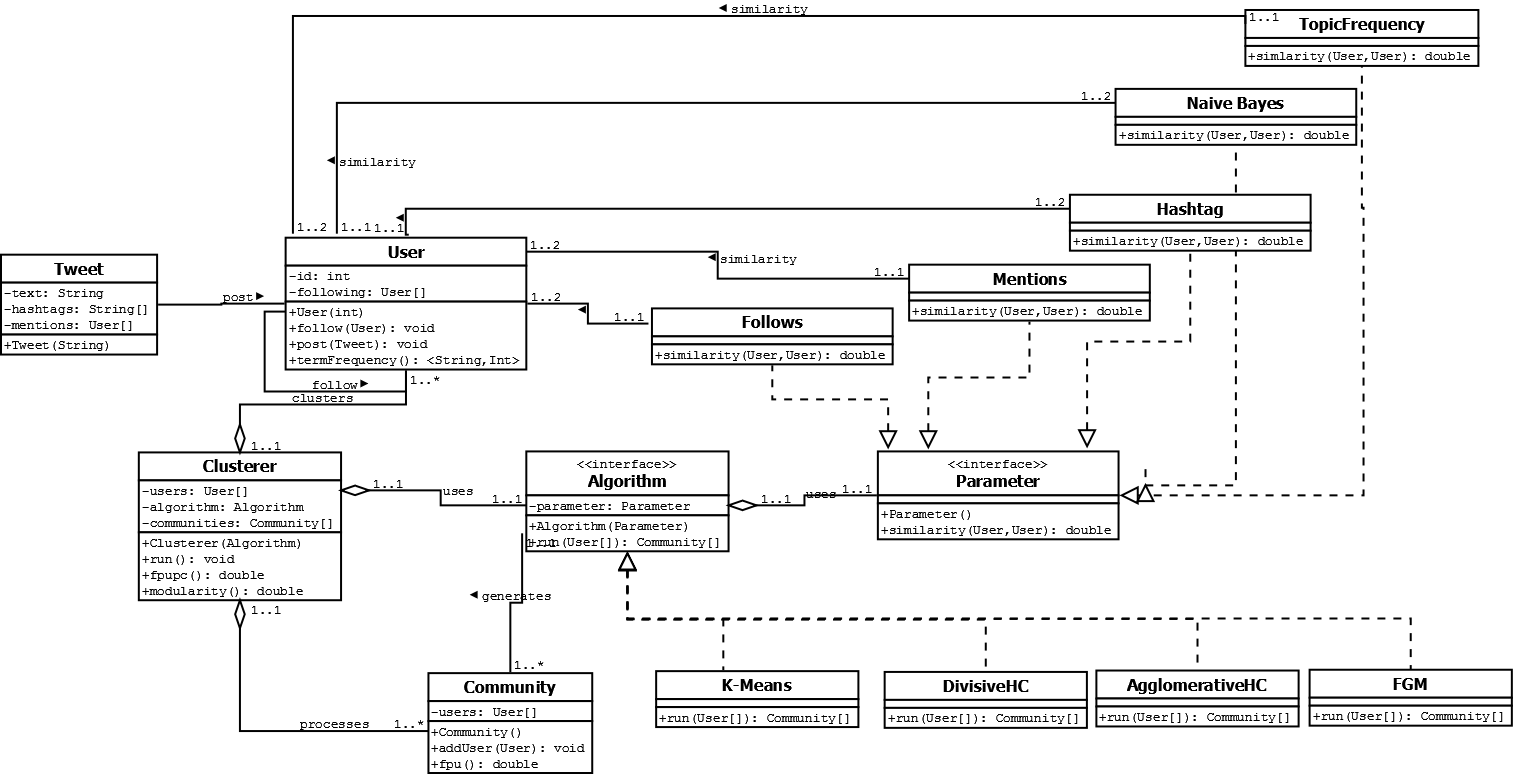
\includegraphics[width=1.4\textwidth]{THS-ST1_FernandezPobleteSanPedroTan_UML_v1}
		\caption{UML Diagram of the Model Component of the Proposed System}
		\label{fig:uml}	
	\end{figure}
\end{landscape}


\newpage


Data collection is done via the \texttt{tweepy} API. The data collection methodology is as follows - three public twitter accounts with a significant amount of followers will be selected. For each account, the first 1000 most recent retrievable tweets will be obtained. Next, a breadth-first search (BFS) will be done for that account\vtick s followers, and their 500 most recent tweets will be retrieved as well. 




The \texttt{UserCrawler.py} file has a function \texttt{get\_all\_tweets(username)}, which is responsible for retrieving the most recent 500 tweets of a particular user, as specified by the username parameter. Initially, three accounts (seeds) will be chosen. Each seed needs to have at least 200 followers. These three seeds are then pushed into a queue. An iterative process then begins, which is described as follows:




At the start of each iteration, a user is popped from the head of the queue. This user’s most recent 500 tweets are collected, and the list of users, representing the account\vtick s followers, is obtained. For each user in that list, the algorithm checks if it has seen that particular user previously. If not, the user is added to the end of the queue.




This iterative process continues until either a depth of 3 in the BFS tree is reached, or a count of 500,000 tweets is reached.




In parallel with the above algorithm, a separate csv file is also generated. This csv file will contain information about the users\vtick following network. Each row of the csv file will begin with the user id of the particular user, followed by the user id\vtick s of all the accounts that user is following.




To anonymize the data, all json elements that may point back to the user are removed. Specifically, these elements are ``name’’, ``description’’, ``profile\_image\_url’’, ``profile\_image\_url\_https’’, ``profile\_background\_image\_url\_https’’, ``profile\_banner\_url’’, and ``profile\_background\_image\_url’’. Additionally, each user id is replaced with an automatically incrementing integer id (starting at 1). This is because the user id can still be mapped to the actual user profile.




For the \texttt{data representation}, this comprises a \texttt{User class} and a \texttt{Tweet class}.


The \texttt{computational model} will have a central class \texttt{Clusterer} which takes a list of users as an attribute, 
as well as an \texttt{Algorithm} object. The algorithm follows the Strategy design pattern, which abstracts the algorithms in
concrete implementations of the \texttt{Algorithm} interface. The \texttt{Algorithm Interface} contains an instance of the \texttt{Parameter interface}
which also follows the Strategy design pattern. In this case, retrieving the similarities between two User objects is abstracted,
to be implemented by the concrete realizations of the Parameter interface. By setting the algorithm and parameter, the \texttt{Clusterer} objects 
runs the algorithm and produces a list of Community objects, which have two derived attributes $modularity$ and $FPUPC$. The \texttt{Clusterer} caches
these Communities and can also return the aggregate $modularity$ and $FPUPC$ of the set of detected communities.


The \texttt{controller} simply interfaces all the model submodules. It checks on startup if the data collection module is done collecting and cleaning data. It passes the data collected, represented as User and Post classes, to the \texttt{Clusterer} class, after setting an algorithm and parameter. This produces the Community objects that the controller then passes as part of the HTTP response.


The \texttt{view module} will be implemented with HTML5, CSS3, and Javascript. 


\section{System Functions}


This section outlines the different functions of the system.


\begin{comment}
\subsection{Collect Data}
\label{us:colldat}


The user prompts the system to collect new data to have a more updated dataset to extract communities from.


Pre-condition: The system is running. (This is automatically run on server startup.)


Scenario:
\begin{enumerate}
\item The user chooses to collect data.
\item The system collects data from Twitter and cleans the data.
\item The system displays a progress bar during this process.
\item The system notifies the user that data collection and cleaning is finished.
\end{enumerate}


Post-condition: The system now has an updated dataset to extract communities from.


Acceptance Criteria:
\begin{itemize}
\item Test if there is stored data. (User story \ref{us:gencom} should output proper communities.)
\item Test if data is clean.
\end{itemize}
\end{comment}


\subsection{Select Algorithm}
\label{us:selectalgo}


The user selects an algorithm in order to set a required parameter for generating communities.


Pre-condition: The system has data from Twitter. The main menu is the current screen.


Scenario:
\begin{enumerate}
	\item The user chooses to select an algorithm.
	\item The system displays all the algorithms (K-Means, Divisive Hierarchical Clustering, Agglomerative Hierarchical Clustering, Fast Greedy Optimization of Modularity) supported by the system.
	\item The user selects one of the algorithms.
	\item The user confirms their choice.
	\item The system redirects to the main menu and displays the selected algorithm as part of the system status.
\end{enumerate}


Post-condition: The system has an algorithm to use for generating communities. The ``Select Parameter'' option
is now enabled in the main menu. The allowed parameters have been enabled in the Select Parameter screen.


Acceptance Criteria:
\begin{itemize}
	\item Test if the algorithm selected is valid.
	\item Test if only one algorithm is selected.
	\item Test if the algorithm is displayed as part of the system status.
	\item Test if the system redirects to the main menu.
	\item Test if the ``Select Parameter'' option is now enabled.
\end{itemize}


\subsection{Select Parameter}
\label{us:selectparam}


The user selects a similarity parameter in order to set a required parameter for generating communities.


Pre-condition: The system has finished collecting data from the data collection module. User story \ref{us:selectalgo} has been finished.


Scenario:
\begin{enumerate}
	\item The user chooses to select a parameter.
	\item The system displays all parameters compatible with the selected algorithm (Follows, Term Frequency, Hashtags, Mentions).
	\item The user selects one parameter to use.
	\item The user confirms their choice.
	\item The system redirects to the main menu with the ``Generate Communities'' option enabled.
\end{enumerate}


Post-condition: The system has a similarity parameter to use for generating communities. The ``Generate Communities'' option
has been enabled in the main menu.


Acceptance Criteria:
\begin{itemize}
	\item Test if the user has already selected an algorithm.
	\item Test if only the parameters compatible with the selected algorithm are displayed in the ``Select Parameter'' screen.
	\item Test if the parameter selected is a valid choice.
	\item Test if only one parameter is selected.
	\item Test if the system redirects to the main menu.
	\item Test if the ``Generate Communities'' option is enabled.
\end{itemize}


\subsection{Generate Communities}
\label{us:gencom}


The user asks the system to generate communities to see the graphical representation of the communities and to see the 
evaluation metrics of the generated communities for the selected algorithm-parameter combination.


Pre-condition: The system has finished collecting data from the data collection module. User stories \ref{us:selectalgo} and \ref{us:selectparam} have been finished.


Scenario:
\begin{enumerate}
	\item The user chooses to generate communities.
	\item The system computes for the communities using the selected algorithm and parameter.
	\item The system displays the graphical representation of the communities as well as the values of the evaluation metrics.
\end{enumerate}


Post-condition: The system is now displaying a graphical representation of the communities and the value of the evaluation
metrics.


Acceptance Criteria:
\begin{itemize}
	\item Test if the user has already selected an algorithm and parameter.
	\item Test if the detected communities are appropriate for the chosen algorithm and parameter.
	\item Test if the evaluation metrics\vtick values are correct.
\end{itemize}


\section{Physical Environment and Resources}
The software was developed using Python as a language and Django as a framework for the web application. Python 3.5 is required to run the code. The web application must be run by a server that supports Django 1.10.1. 




               %-- includes LaTeX source file for Chapter 3: Research Methodology
								  %-- your job: **EDIT THIS FILE** to indicate your research methodology


\appendix                         %-- used to specify appendices
%%%%%%%%%%%%%%%%%%%%%%%%%%%%%%%%%%%%%%%%%%%%%%%%%%%%%%%%%%%%%%%%%%%%%%%%%%%%%%%%%%%%%%%%%%%%%%%%%%%%%%%
%
%   Filename    : appendix_A.tex 
%
%   Description : This file is one of the appendices. 
%                 
%%%%%%%%%%%%%%%%%%%%%%%%%%%%%%%%%%%%%%%%%%%%%%%%%%%%%%%%%%%%%%%%%%%%%%%%%%%%%%%%%%%%%%%%%%%%%%%%%%%%%%

\chapter{Diagrams and Other Documentation Tools}
\label{sec:appendixa}


This appendix may consist of proposed architectural design, algorithms, scientific formula for 
MSCS and Data Flow Diagrams, Fishbone for MSIT.


              %-- includes LaTeX source file for Appendix A
                                                 %-- your job: **CREATE/EDIT** your own source file for the appendices
	%%%%%%%%%%%%%%%%%%%%%%%%%%%%%%%%%%%%%%%%%%%%%%%%%%%%%%%%%%%%%%%%%%%%%%%%%%%%%%%%%%%%%%%%%%%%%%%%%%%%%%
%
%   Filename    : appendix_B.tex 
%
%   Description : This file will contain one of your appendices.
%                 
%%%%%%%%%%%%%%%%%%%%%%%%%%%%%%%%%%%%%%%%%%%%%%%%%%%%%%%%%%%%%%%%%%%%%%%%%%%%%%%%%%%%%%%%%%%%%%%%%%%%%%

\chapter{Research Ethics Documents}
\label{sec:appendixb}

This section contains the research ethics documents related to this research proposal.



%%%%%%%%%%%%%%%%%%%%%%%%%%%%%%%%%%%%%%%%%%%%%%%%%%%%%%%%%%%%%%%%%%%%%%%%%%%%%%%%%%%%%%%%%%%%%%%%%%%%%%
%
%   Filename    : appendix_C.tex
%
%   Description : This file will contain information about your Resource Persons
%                 
%%%%%%%%%%%%%%%%%%%%%%%%%%%%%%%%%%%%%%%%%%%%%%%%%%%%%%%%%%%%%%%%%%%%%%%%%%%%%%%%%%%%%%%%%%%%%%%%%%%%%%

\chapter{Resource Persons}
\label{sec:appendixc}

%
%  Indicate your resource persons here:
%
%	<full name and title, e.g., Dr. Juan de la Cruz>
%	<profession, e.g., faculty>
%	<department, e.g., College of Computer Studies>
%	<name of institution, e.g., De La Salle University>
%	<e-mail address>
%
%

%
%  the following shows 3 examples, replace entries with your own
%
\newcommand{\resperson}[4]{\textbf{#1} \\ #2 \\ #3 \\ \url{#4}\vspace{0.5em}\\}

\resperson{Ms. Charibeth Cheng}{Adviser}{College of Computer Studies\\De La Salle University-Manila}{chari.cheng@delasalle.ph}
%\resperson{Mr. Firstname2 Lastname2}{Role2}{Affiliation2}{emailaddr2@domain.com}
%\resperson{Ms. Firstname3 Lastname3}{Role3}{Affiliation3}{emailaddr3@domain.net}




%\bibliographystyle{apacite}       %-- specified APA style for bibliograpy
                                  %-- more details about APA style citation can be found in www.ctan.org/tex-archive/biblio/bibtex/contrib/apacite/

                                  %-- bibliographic entries are handled via bibtex; refer to www.bibtex.org for more details

\bibliography{myreferences}       %-- the file "myreferences.bib" is a sample bibliography (bib) from SIGGRAPH 
                                  %-- your job: **CREATE/EDIT** your own bibliography file  

\end{document}

